% Table des matières :


% - Présentation
% - Délimitation du sujet
% - Problématique

% I - Cadre théorique
% - Modéliser un espace réel en informatique
% Description ensembliste : ensemble convexe
% Théorie des graphes : Algorithme de plus court chemin
% - Algorithme retenue : A* ou Dijkstra étentue
% Définition du graphe
%     structure
%     Noeud
%     Evalution euristique du noeud + Distance (euclide/Manhatann)
%     relation d'ordre sur les noeuds (egalité et supérieur)
% Présentation du principe : distance utilisé (manathan/Euclide)

% II - Implémentation

% Choix du langage : Python/Ocaml
% représentation du graphe en Python
%     dico ou matrice : dico pour simplicité d'écriture
% Implémentation :
%     noeuds
%     relation d'ordre
%     Fonction auxiliaire
% Choisir le meilleur noeud : On tri la liste ou on utilise une structure de tas
 
% Comparaison des implémentation : 
% fonction de comparaison
% Différence

% Influence du choix de l'évaluation heuristique (Vitesse/Précision)

% Complexité temporelle de l'Algorithme

% III - Experimentation en condition réelle

% Présentation contexte Robocup et de l'expérience
% Présentation du robot (pourquoi ces robots)

% Mise en place de l'experience
%     Dispositif physique

%     Dispositif informatique
%         Module Holobot
%         Analyse d'image

% Résultat : 
% Commande du robot non optimal provoque lenteur d'execution
% Ouverture : Modéliser des trajectoires a partir du chemin
%             pour plus de fluidité

\usepackage{graphicx}
\usepackage{siunitx}

\newtheorem{definition}{Définition}
\newtheorem{proposition}{Proposition}
\newtheorem{proof}{Démonstration}


\begin{document}

\maketitle

\newpage
\tableofcontents
\newpage

\section{Introduction}
Ce travail s’inscrit dans le cadre du travail d’initiative personnel encadré demandé en classe préparatoire aux grandes écoles. 
Le thème de ce travail est « Enjeux sociétaux ».
Le sujet abordé est la recherche de chemins. Ce procédé permet de répondre à des problématiques concrètes telles que le traçage de route 
avec des contraintes de zone non constructible tout en optimisant les temps de trajet. Les enjeux sont alors des enjeux environnementaux 
et énergétiques.
La détermination de chemin fait partie du champ de recherche lié à la navigation et à l’intelligence artificielle. Elle est devenue un 
sujet très important avec le développement de la robotique.
Le besoin de chercher un chemin est de plus en plus important. En effet, il est utile pour tracer des routes entre deux villes, 
gérer les chemins de connexion entre deux téléphones ou encore tracer des pistes sur une carte électronique.

La théorie des graphes est un bon outil pour ce genre de problème. Son origine remonte au XVIIIe siècle avec le problème des 
sept ponts de Königsberg (aujourd’hui Kaliningrad en Russie). Ce problème consiste à déterminer s’il existe une promenade, 
en partant d’un point de départ au choix, dans les rues de la ville qui permet de ne passer qu’une seule fois sur chaque pont 
et de revenir au point de départ. Ce problème a été résolu par Euler et une démonstration rigoureuse a été formulée en 1873 qui 
conclut qu’une telle promenade n’existe pas. Cependant, d’autres formes de modélisation ont émergé notamment des modélisations 
reposant sur l’étude des ensembles non convexe.

Depuis ces modélisations, de nombreux algorithmes ont été réalisés. Avec la modélisation reposant sur les ensembles non convexes 
viennent des algorithmes d’exploration comme le « Rapidly-exploring random tree ». Avec les modélisations liées aux graphes vient 
des algorithmes comme le « A* » ou l’algorithme de Dijkstra. 

La recherche dans ce domaine est très active. C’est le cas avec la compétition internationale de robotique : la « RoboCup ». 
De nombreuses équipes de plusieurs pays se réunissent chaque année autour de la robotique avec pour objectif en 2050 de mettre au point une équipe de football constitué de robots humanoïdes capable de battre une équipe humaine. Dans ce cadre, de nombreux chercheurs travaillent et organisent lors de l’évènement des matchs entre équipes robotiques. Le groupe de chercheur le plus avancé actuellement est le groupe de la Rhoban de Bordeaux, membre du « LABRI » cumulant en 2020 quatre titres de champion du monde. La RoboCup est maintenant diversifiée avec de nouveaux challenges, notamment, la ligue « Small Size League » (SSL) qui oppose deux équipes de 6 ou 12 robots à roues.
Une approche de ce problème peut être abordée par une implémentation en Python d’un algorithme de recherche de chemin. 
Cet algorithme peut ensuite être utilisé avec un système de reconnaissance d’image et un robot à roues holonomes.

L’enjeu de trouver des chemins est alors primordial dans beaucoup de domaines et particulièrement en robotique. 
Il est donc nécessaire de trouver comment permettre la navigation d’un robot de la ligue SSL sur un terrain de football.

\section{Théorie}

\subsection{Description ensembliste}

La première étape est de choisir une façon de modéliser un terrain de football. Afin de le décrire, plusieurs méthodes peuvent 
être utilisées. 
Premièrement vient une description ensembliste du terrain. Cela revient alors à caractériser le terrain comme un ensemble de 
points. De plus, certains points peuvent ne pas être accessibles. Ils sont alors enlevés de l’ensemble.

\begin{center}
    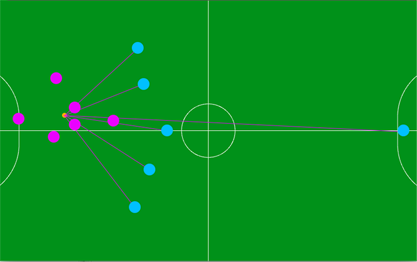
\includegraphics[height=7cm]{4.png}
\end{center}

\begin{definition} Ensemble convexe \\
    On dit qu'un ensemble $A$ est convexe lorsque : \\
$\forall X,Y \in A, \forall t \in [0,1], tx+(1-t)y \in A$
\end{definition}

\begin{definition} Ensemble connexe par arcs \\
    On dit que $A$ est connexe par arcs lorsque : \\
    $\forall X,Y \in A,\exists \varphi \in \mathcal{C}([0,1],A),\forall t \in [0,1], \begin{cases} \varphi(0)=X, & \mbox{ }  \\ \varphi(1)=Y, & \mbox{ }\mbox{ }\\\forall t \in [0,1], \varphi(t) \in A, & \mbox{ } \mbox{ } \end{cases}$
\end{definition}

\begin{definition} Chemin \\
    On appelle chemin dans un ensemble $A$ une suite de point de A.
\end{definition} 

On constate alors que si l’ensemble est convexe, le chemin optimal est une ligne droite. Dans le cas contraire, un ensemble 
connexe par arcs assure l’existence d’un chemin. Cependant, cette méthode est une méthode pouvant être appelée continue. 
En effet, il y a une infinité de points dans un tel ensemble. Cette méthode n’est donc pas, dans une première mesure, 
adaptée dans notre contexte.

\subsection{Théorie des graphes}

Une autre modélisation repose alors sur la théorie des graphes. Cette théorie permet une modélisation adaptée à l’informatique. 
Il est alors plus abordable d’écrire un algorithme de recherche de chemin.
L’algorithme retenu est alors l’algorithme « A* ». 
Nous allons premièrement définir le graphe utilisé puis nous reviendrons sur le principe de cet algorithme.
Le graphe utilisé peut être assimilé à une matrice. Chaque coefficient de cette matrice correspond à un nœud. 
On note dans la suite $L$,$H$ respectivement le nombre de colonnes et le nombre de lignes de cette matrice. On note $\mathcal{S}$ 

\begin{definition} Évaluation Heuristique \\
    On appelle évaluation heuristique une $\mathcal{H} : \mathcal{S} \longrightarrow \mathbb{R}$.
\end{definition} 

\begin{definition} Nœud \\
    On appelle coordonnée $C \in [\![0,L[\![ \times [\![0,H[\![$ \\
    On note $D_d$ la distance au nœud de départ \\
On note $D_a$ la distance au nœud d’arrivé \\
On note $\mathcal H$ l’évaluation heuristique du nœud \\
On appelle nœud le quadruplet $(C,D_d,D_a,\mathcal H)$ \\
\end{definition}

L’évaluation heuristique d’un nœud est une façon de donner un cout à un nœud. Elle peut par exemple être la somme $D_d+D_a$.

\begin{definition}
    On dit que deux nœuds $N_1$,$N_2$ sont égaux lorsqu’ils ont les mêmes coordonnées. On note alors $N_1 = N_2$. \\
On dit qu’un nœud $N_1$ est inférieur à un nœud $N_2$ lorsque le cout de $N_1$ est inférieur à celui de $N_2$. On note $N_1<N_2$.

\end{definition}

Le principe de l’algorithme est proche des algorithmes classiques. On partitionne les nœuds en deux ensembles :  D et A. 
D contient les nœuds visités tandis que A contient les nœuds à visiter. On sélectionne premièrement le nœud dans A avec 
le cout le plus bas. On visite ensuite les voisins directs de ce nœud. On calcule alors son cout. Si un voisin à un cout 
plus faible que tous les autres nœuds de A, on l’ajoute dans A. l’algorithme se termine lorsque le nœud final est visité. 
Il est alors possible de déterminer un chemin entre le nœud de départ et le nœud final.

\section{Implémentation}
\subsection{Implémentations}

Le choix du langage pour implémenter cet algorithme est très important. Dans le cadre du programme, 
les deux langages utilisables sont Python et Ocaml. Notre but est d’implémenter l’algorithme sur un robot. 
Nous avons choisi d’utiliser Python afin de bénéficier de sa flexibilité et d’un grand nombre de modules disponibles.
Nous avons choisi de représenter un nœud dans un premièrement uniquement avec ses coordonnées. 
Implémenter le graphe revient alors à stocker un ensemble de couples. Nous utiliserons un dictionnaire afin de bénéficier 
d’une syntaxe plus limpide que celle des tableaux de tableaux.


Afin d’implémenter les nœuds et les relations, nous utilisons une classe Nœud :

\begin{minted}[
    frame=lines,
    framesep=2mm,
    baselinestretch=1.2,
    bgcolor=white,
    fontsize=\footnotesize,
    linenos]
    {Python}
class Noeud:
	def __init__(self, position:(), parent:()):
		self.position = position
		self.parent = parent
		self.g = 0 # Distance au Noeud de départ
		self.h = 0 # Distance au Noeud de fin
		self.f = 0 # Cout total
	def __eq__(self, other):
		return self.position == other.position
	def __lt__(self, other):
		return self.f < other.f
\end{minted}

Nous utilisons aussi quelques fonctions auxiliaires.

On peut réaliser une fonction qui indique si un nœud doit être ajouté dans la liste des nœud à visiter, c’est-à-dire s’il 
n’est pas déjà dans la liste et si son cout est inférieur au cout des autres nœuds de la liste. On a alors :

\begin{minted}[
    frame=lines,
    framesep=2mm,
    baselinestretch=1.2,
    bgcolor=white,
    fontsize=\footnotesize,
    linenos]
    {Python}
def add_to_à_Visiter(à_visiter, voisin):
    for noeud in à_visiter:
      if (voisin == noeud and voisin.f >= noeud.f):
        return False
    return True
\end{minted}

On réalise aussi une fonction qui calcul la distance entre deux nœuds. On a :

\begin{minted}[
    frame=lines,
    framesep=2mm,
    baselinestretch=1.2,
    bgcolor=white,
    fontsize=\footnotesize,
    linenos]
    {Python}
def Distance(a,b):
    return ((b.position[0]-a.position[0])**2 + (b.position[1]-a.position[1])**2)**(1/2)
\end{minted}

Enfin, on réalise une fonction qui prend en entrée un tableau de tableaux et qui renvoie les paramètres initiaux pour l’algorithme final. 
On a :

\begin{minted}[
    frame=lines,
    framesep=2mm,
    baselinestretch=1.2,
    bgcolor=white,
    fontsize=\footnotesize,
    linenos]
    {Python}
def carteFromMatrix(M):
    largeur = len(M[0])
    hauteur = len(M)
    map = {}
    deb,fin = (0,0),(0,0)
  
    for j in range (hauteur):
      for i in range (largeur):
        map[(i, j)] = M[j][i]
        if M[j][i]=='@':
          deb = (i,j)
        if M[j][i]=='$':
          fin = (i,j)
  
    return map,deb,fin,largeur,hauteur
\end{minted}


Il est alors maintenant possible d’implémenter une première version de l’algorithme.
Dans cette première implémentation, on utilisera deux tableaux pour stocker les nœuds déjà visités et les nœuds à visiter. 
Pour simplifier la sélection du meilleur nœud, on triera la liste des nœuds à visiter .

\begin{minted}[
    frame=lines,
    framesep=2mm,
    baselinestretch=1.2,
    bgcolor=white,
    fontsize=\footnotesize,
    linenos]
    {Python}
def A_étoile(map, deb, fin):
	à_visiter = []
	déjà_vu = []
	start_node = Noeud(deb, None)
	goal_node = Noeud(fin, None)
	à_visiter.append(start_node)

	while len(à_visiter) > 0:
		à_visiter.sort()																							# TODO : Utiliser un tas?
		current_node = à_visiter.pop(0)
		déjà_vu.append(current_node)

		if current_node == goal_node:
			path = []
			while current_node != start_node:
				path.append(current_node.position)
				current_node = current_node.parent
			return path

		(x, y) = current_node.position
		# On liste ces voisins
		Voisins = [(x-1, y), (x+1, y), (x, y-1), (x, y+1)]

		for next in Voisins:
			map_value = map.get(next)
			if(map_value == '#'):
				continue
			voisin = Noeud(next, current_node)
			if(voisin in déjà_vu):
				continue
			voisin.g = Distance(voisin,start_node)
            voisin.h = Distance(voisin,goal_node)

			voisin.f = voisin.g + voisin.h

			if(add_to_à_Visiter(à_visiter, voisin) == True):
				à_visiter.append(voisin)
	return None
\end{minted}



L’inconvénient de cette méthode est qu’il est nécessaire de trier la liste à chaque ajout d'un nouveau nœud. 
Il est alors intéressant d’utiliser une structure de tas pour simplifier la sélection. On utilise le module «headp» qui 
implémente les tas en Python. 
On obtient alors :

\begin{minted}[
    frame=lines,
    framesep=2mm,
    baselinestretch=1.2,
    bgcolor=white,
    fontsize=\footnotesize,
    linenos]
    {Python}
def A_étoile(map, deb, fin):
    à_visiter = []
    déjà_vu = []
    start_node = Noeud(deb, None)
    goal_node = Noeud(fin, None)
    heapq.heappush(à_visiter,start_node)
  
    while len(à_visiter) > 0: 
      current_node = heapq.heappop(à_visiter)
      déjà_vu.append(current_node)
  
      if current_node == goal_node:
        path = []
        while current_node != start_node:
          path.append(current_node.position)
          current_node = current_node.parent
        return path
  
      (x, y) = current_node.position
      Voisins = [(x-1, y), (x+1, y), (x, y-1), (x, y+1)]
  
      for next in Voisins:
        map_value = map.get(next)
        if(map_value == '#'):
          continue
        voisin = Noeud(next, current_node)
        if(voisin in déjà_vu):
          continue
        voisin.g = Distance(voisin,goal_node)
        voisin.h = Distance(voisin,start_node)
  
        voisin.f = voisin.g + voisin.h
        if(add_to_à_Visiter(à_visiter, voisin) == True):
          heapq.heappush(à_visiter,voisin)
  
    return None
\end{minted}



\subsection{Comparaison}

On se propose de réaliser un programme qui compare le temps d’exécution des deux algorithmes précédents. 
De plus on réalisera une fonction qui créer des tableaux de tableaux aléatoirement afin de tester les algorithmes 
sur les mêmes tableaux avec des obstacles aléatoires. On obtient : 
\begin{center}
    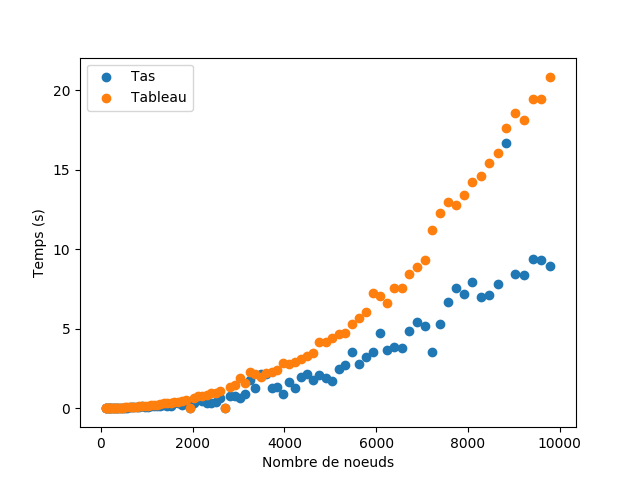
\includegraphics[height=7cm]{1.png}
\end{center}


On constate que la version utilisant un tas est plus efficace que la version utilisant une liste. 
Cependant, on peut se rendre compte que la complexité sera toujours polynomiale.
Nous utiliserons dans la suite la version avec le tas.

\subsection{Évaluation Heuristique}

Nous pouvons maintenant modifier l’évaluation heuristique et mesurer la différence de précision et de rapidité. 
Les deux évaluations prises en compte sont la somme des distances entre le nœud de départ et final et la distance 
au nœud final. 
On obtient pour le temps d’exécution le graphe suivant :

\begin{center}
    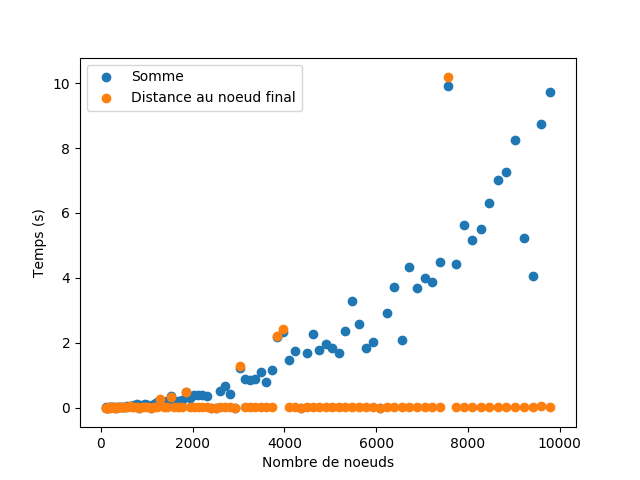
\includegraphics[height=7cm]{2.png}
\end{center}

On constate alors que l’évaluation à un impact directe sur la rapidité du programme. Cela peut venir de 
la précision de l’algorithme. En effet, il est possible de caractériser la précision de l’algorithme par la longueur 
du chemin trouvé. 
Nous mesurons alors la longueur du chemin en fonction du nombre de nœuds du graphe. 

On obtient alors le graphe suivant :

\begin{center}
    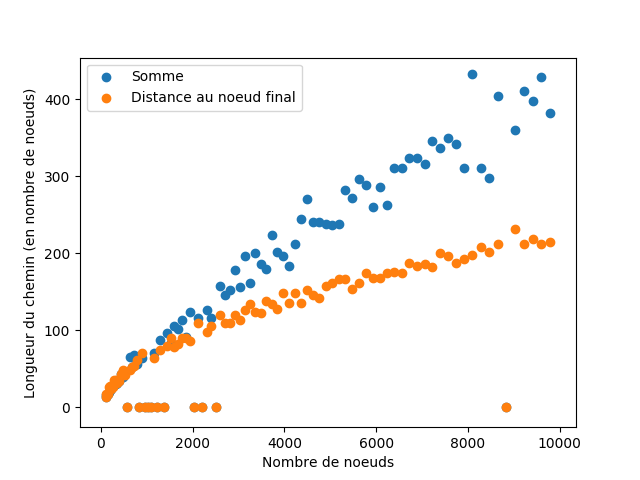
\includegraphics[height=7cm]{3.png}
\end{center}

L’hypothèse est alors validée. L’évaluation la plus efficace est alors celle qui ne dépend que de la distance du 
nœud au nœud final. 

\subsection{Complexité}

En intelligence artificielle, il peut être difficile d’exprimer la complexité temporelle en fonction d’un nombre de sommets et 
du nombre d’arrêtes. En effet, ces nombres sont très grands et il n’est pas question de visiter tous les sommets du graphe. 
Donner la complexité en fonction du nombre de sommet et d’arrêtes n’a alors que peu de sens. La quantité importante est alors 
le nombre de sommets visités et non le nombre de sommets que comporte le graphe.
Il convient alors de définir plusieurs paramètres. Le premier est le facteur d’embranchement. Il s’agit du nombre de voisins de 
chaque nœud. Dans notre algorithme, ce nombre vaut 4. Le second est la profondeur du nœud final. Il s’agit de la longueur du chemin 
solution.
Ces paramètres sont nommés ainsi, car le graphe exploré peut être représenté comme un arbre. Cet arbre est alors un graphe inclus 
dans le graphe initial.
Il est alors plus adéquat de calculer la complexité dans cet arbre plutôt que dans le graphe complet.
Il s’agit alors de déterminer le nombre de sommets dans un arbre de facteur d’embranchement $b$.

\begin{proposition}
    Soit $n \in \mathbb{N}$. Le nombre de nœuds de profondeur $n$ dans un arbre de facteur d'embranchement $b$ est $b^n$
\end{proposition}

\begin{proof}
    $\forall n \in \mathbb{N},$ notons $\mathcal{P}_n$ : " Le nombre de nœud de profondeur $n$ est $b^n$" \\
    \begin{itemize}
        \item Le nombre de nœuds de profondeur $0$ est $b^0=1$. Soit $\mathcal{P}_0$
        \item On suppose $\mathcal{P}_n$ pour un certain $n\in\mathbb{N}$ fixé. Chaque nœud a $b$ fils. Alors à chaque nœud de profondeur $n$ correspond $b$ nœud de profondeur $n+1$. Le nombre de nœuds de profondeur $n+1$ est alors $b^n\cdot b=b^{n+1}$. Soit $\mathcal{P}_{n+1}$
        \item D'après le principe de récurrence, pour tout $n \in \mathbb{N}$, le nombre de nœuds de profondeurs $n$ est $b^n$
    \end{itemize}
\end{proof}

En notant b le facteur d’embranchement et p la profondeur du nœud final la complexité de l’algorithme est alors $O(b^p)$



\section{Expérimentation}

Ce travail d’initiative personnel encadré a été réalisé dans le but de répondre à une problématique. Il s’agit de trouver un 
chemin entre deux points afin de permettre à un robot de se déplacer sur un terrain.
La première étape est de mettre en place le dispositif. Il s’agit d’une caméra filmant un robot d’en haut afin de le repérer 
dans un système de coordonnées. 

INSERT PHOTO MONTAGE

Les robots utilisés sont les robots « Holobots » développés par la Rhoban de l’université de 
Bordeaux et plus précisément le LABRI.

INSERT PHOTO ROBOT

Nous avons choisi ces robots pour leurs roues holonomes. Il s’agit de roues permettant des déplacements dans toutes les 
directions du plan. Elles sont très utiles afin de ne pas utiliser de rotation et de ne pas devoir repérer le sens de déplacement 
du robot. Cela permet de repérer le robot par un point.

INSERT PHOTO ROUE HOLO


Afin de repérer le robot, nous avons programmé un système de reconnaissance d’image. Ce programme utilise la bibliothèque « OpenCV ».

\begin{minted}[
    frame=lines,
    framesep=2mm,
    baselinestretch=1.2,
    bgcolor=white,
    fontsize=\footnotesize,
    linenos]
    {Python}
def analyse(frame):
    x,y=-1,-1
    flag = False

    frame = imutils.resize(frame, width=tailleImage)
    hsv = cv2.cvtColor(frame, cv2.COLOR_BGR2HSV)
    mask = cv2.inRange(hsv, orangeLower, orangeUpper)

    cnts = cv2.findContours(mask.copy(), cv2.RETR_EXTERNAL, cv2.CHAIN_APPROX_SIMPLE)[-2]
    center = None

    if len(cnts) > 0:
        c = max(cnts, key=cv2.contourArea)
        ((x, y), radius) = cv2.minEnclosingCircle(c)

        if radius > 10:
            cv2.circle(frame, (int(x), int(y)), int(radius), (0, 255, 255), 2)
            flag = True
        else:
            radius = -1
            x = -1
            y = -1
            flag = False
    else:
        radius = -1
        x = -1
        y = -1
        flag = False

    return  flag,(x,y),frame,mask
\end{minted}

Il est alors très simple d’implémenter l’algorithme A* en utilisant le module Metabot de la Rhoban.

\begin{minted}[
    frame=lines,
    framesep=2mm,
    baselinestretch=1.2,
    bgcolor=white,
    fontsize=\footnotesize,
    linenos]
    {Python}
holo = Holobot(sys.argv[1], 115200)
camera = cv2.VideoCapture(0)

def deplacement_élémentaire(pos, dest ,poids=30 ,tps=0.1):
    x=dest[0]-pos[0]
    y=dest[1]-pos[1]
    
    holo.control(poids*x,poids*x,0)
    time.sleep(tps)

def deplacement():
    (grabbed, frame) = camera.read()
    B,coord,frame,mask = analyse(frame)
    mat = nvmat(len(mask),len(mask[0]))
    map,deb,fin,largeur,hauteur = carteFromMatrix(mat)
    path = A_étoile(map,deb,fin)
    dest=path[1]
    x=coord[0]
    y=coord[1]
    if x>=0 and y>=0:
        deplacement(coord, dest)
\end{minted}

INSERT PHOTO IMAGE CAMERA

Le problème rencontré est que le chemin est discret. En effet le robot se déplace alors de point en point de façon saccadée. 
Une solution peut être de modéliser des trajectoires à partir de ces points afin d’avoir des déplacements continus et plus de fluidité.

\end{document}